 \thispagestyle{gocconone}
\pagestyle{gocco}
\everymath{\color{gocco}}
\graphicspath{{../gocco/pic/}}
\blfootnote{$^1${\color[named]{gocco}Trung tâm Ứng dụng Công nghệ Vũ trụ Tp. Hồ Chí Minh.}}
\begingroup
\AddToShipoutPicture*{\put(0,616){\includegraphics[width=19.3cm]{../bannergocco}}}
\AddToShipoutPicture*{\put(120,525){\includegraphics[scale=1]{../tieude2.pdf}}} 
\centering
\endgroup

\vspace*{185pt}
\begin{multicols}{2}	
	Đối với các tình huống trên bàn cờ, ta thường đánh giá tình hình dựa vào $2$ yếu tố: \textit{Quân} (tương quan lực lượng của đôi bên) và \textit{Thế} (vị trí, sự liên kết giữa các quân). Nhìn chung, những yếu tố này bù đắp, hỗ trợ những khiếm khuyết, ưu -- nhược điểm của nhau. Tuy nhiên, nhiều nhà nghiên cứu lý luận Cờ Tướng đã đồng ý thống nhất rằng, yếu tố \textit{Thế} ảnh hưởng nhiều hơn đến kết quả của cuộc cờ. Trong diễn biến mỗi ván đấu, nếu như những nước đi, các biến hóa của Khai cuộc thường mang nặng tính lý thuyết, đa phần dựa vào những nước đi đã được nghiên cứu theo sách vở và phần mềm, thì những giai đoạn tiếp theo phụ thuộc nhiều vào trình độ cũng như khả năng tính toán của đôi bên. Muốn có được thế tốt trong Trung, Tàn cuộc để hướng tới một kết quả có lợi thì vấn đề điều chuyển quân, hay còn được gọi là \textit{Điều động lực lượng} là một yêu cầu vô cùng quan trọng.
	\vskip 0.1cm
	\textit{Điều động lực lượng} được xem là thời điểm chuyển đổi trạng thái giữa các tình  huống, đó cũng có thể được coi là giai đoạn bước ngoặt, quyết định kết quả sau cùng của mỗi ván đấu. Vì vậy, đòi hỏi các kỳ thủ cần phải nắm rõ đâu là vị trí mấu chốt của cuộc cờ, đồng thời cần có một kế hoạch chi tiết, cụ thể mới có thể đưa những quân lực ở vào những vị trí thuận lợi nhất. 
	\vskip 0.1cm
	Để cụ thể hơn về chủ đề \textit{Điều động lực lượng}, tác giả sẽ gửi tới bạn đọc Pi vài ví dụ tiêu biểu có thể áp dụng vào những tình huống trong thực chiến.
	\begin{figure}[H]
		\vspace*{-5pt}
		\centering
		\captionsetup{labelformat= empty, justification=centering}
		\includegraphics[width= 0.4\textwidth]{1}
		\caption{\small\textit{\color{gocco}Hình $1$.}}
		\vspace*{-10pt}
	\end{figure}
	$1.$ Hình $1$, Quân lực tấn công của đôi bên hoàn toàn tương đồng, Đen đang hơn $1$ Sỹ. Tuy nhiên hệ thống Mã và $2$ Sỹ của Đen đang bị giam chặt bởi Pháo đỏ, Đỏ được quyền đi trước và vận dụng triệt để nghệ thuật Điều động lực lượng để giành chiến thắng như sau:
	\vskip 0.1cm
	$\pmb{1)}$ M$6.7$ P$2-3$\quad  $\pmb{2)}$ S$5.4$ Tg$6.1$\quad $\pmb{3)}$ P$8/8$ Tg$6/1$$(*)$ \quad$\pmb{4)}$ P$8-4$ P$3-6$\quad  $\pmb{5)}$ S$4/5$ P$6-3$$(**)$ \quad$\pmb{6)}$ M$7/5$ M$4.5$\quad $\pmb{7)}$ M$5.3$ M$5/7$\quad  $\pmb{8)}$ M$3/4$ S$5.6$\quad $\pmb{9)}$ M$4.6$ S$6/5$\quad $\pmb{10)}$ M$6.7$$(***)$ (Đen mất Pháo, chắc chắn thua cuộc)
	\vskip 0.1cm
	\textit{$(*)$: Nhận ra điểm yếu, Đỏ lập tức lao Mã tới bắt Mã Đen, buộc Đen phải bình Pháo cản khiến cho cả đội hình của Đen kẹt cứng, chỉ có thể di chuyển Tướng. Đỏ tiếp tục giương Sỹ làm ngòi rồi thoái Pháo về đáy dọa sát.
	\vskip 0.1cm
	$(**)$: Đỏ liên tục bình Pháo rồi thoái Sỹ uy hiếp. Để tránh mất quân, Đen lại phải bình Pháo về chỗ cũ. Như vậy sau vài nước điều quân cực kỳ mẫu mực của Đỏ, Đội hình của Đen vẫn không có gì thay đổi.
	\vskip 0.1cm
	$(***)$: Sau khi đem Pháo về vị trí chiến lược, Đỏ tiếp tục có những nước điều động Mã uy hiếp đầy uy lực. Đen đã rất cố gắng chống đỡ nhưng cuối cùng đành chấp nhận thất bại.}
	\begin{figure}[H]
		\vspace*{-5pt}
		\centering
		\captionsetup{labelformat= empty, justification=centering}
		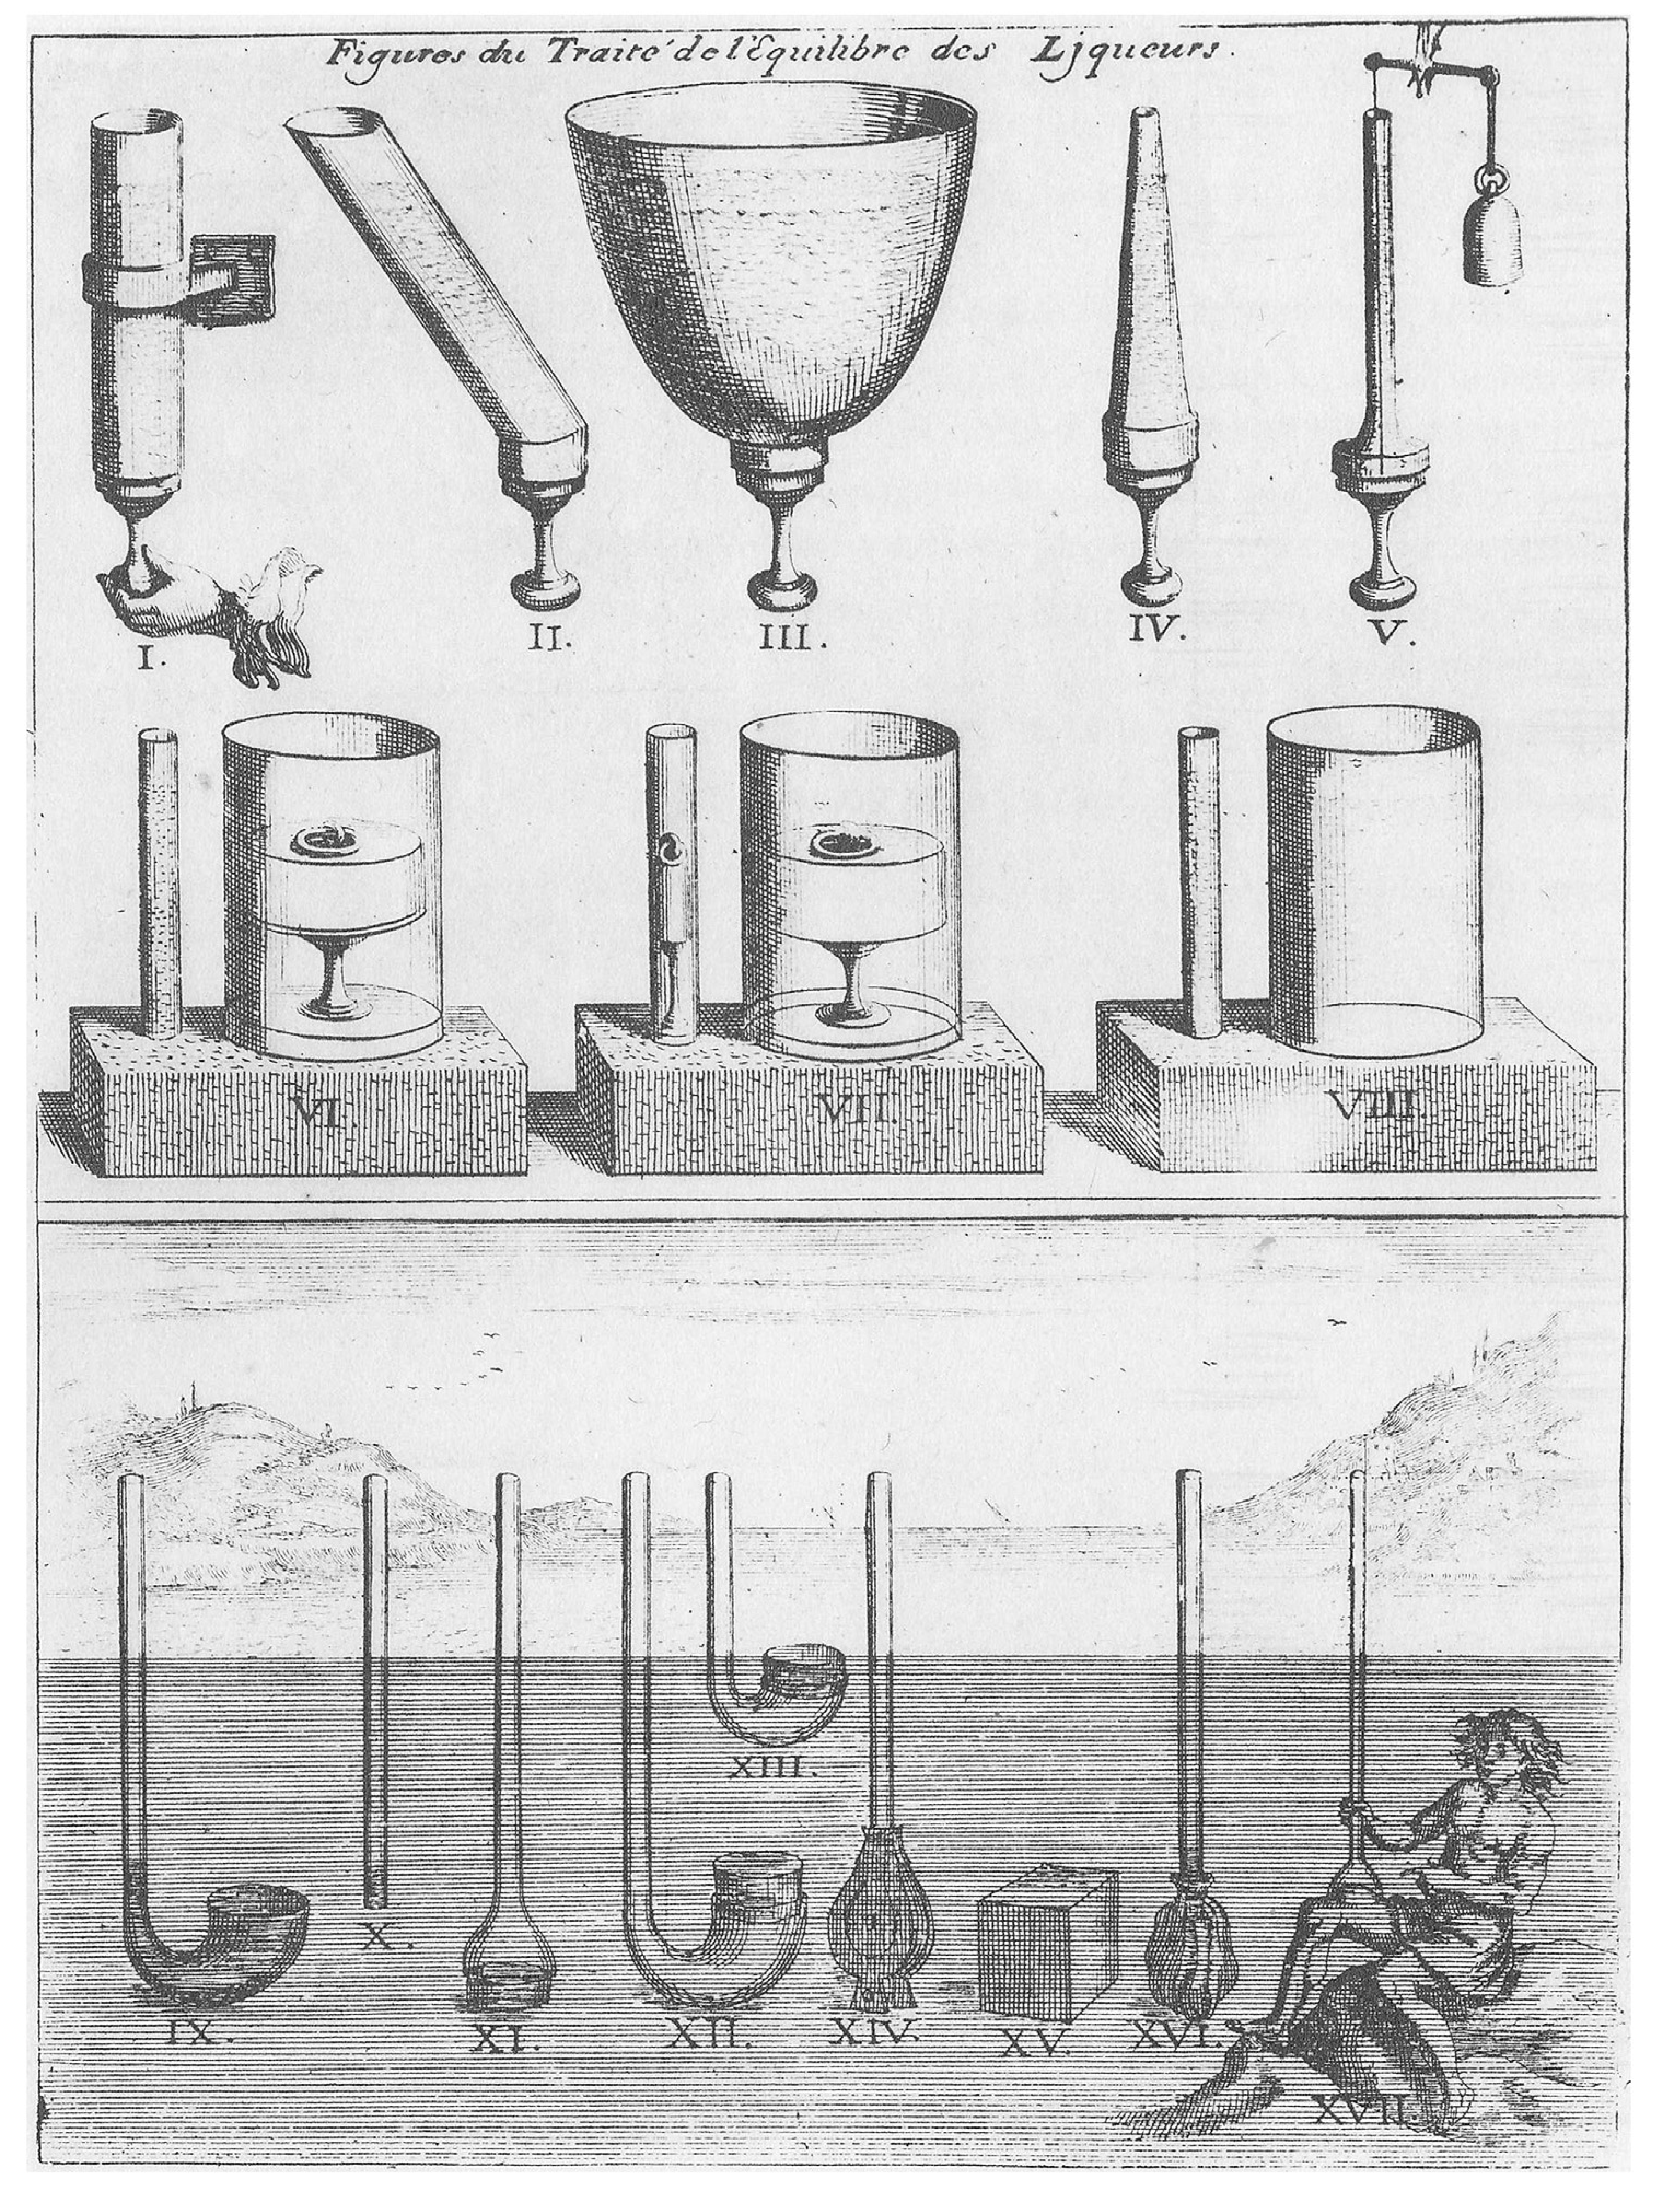
\includegraphics[width= 0.4\textwidth]{2}
		\caption{\small\textit{\color{gocco}Hình $2$.}}
		\vspace*{-10pt}
	\end{figure}
	$2.$ Hình $2$, thoạt nhìn có thể thấy Đen còn chiến Xe và Chốt áp sát rất mạnh, Đỏ chỉ Pháo, Mã, Chốt đang ở những vị trí không thuận lợi cho lắm. Nếu sắp tới Đỏ không có những động thái rõ ràng, Đen sẽ nhanh chóng giành thắng lợi. Tuy nhiên, Đỏ được quyền đi trước và liên tục có những nước đi chính xác như sau:
	\vskip 0.1cm
	$\pmb{1)}$	M$5/3$ Tg$6/1$\quad $\pmb{2)}$ P$5-1$ M$5.7$$(*)$\quad  $\pmb{3)}$ P$1.1$ Tg$6/1$\quad $\pmb{4)}$ M$3.4$  M$7.5$$(**)$\quad  $\pmb{5)}$ C$2-3$ Tg$6.1$\quad $\pmb{6)}$ M$4.2$ M$5/7$\quad $\pmb{7)}$ P$1-3$ X$4/1$$(***)$\quad $\pmb{8)}$ M$2/3$ Tg$6.1$\quad $\pmb{9)}$ P$3-1$ X$4-7$\quad $\pmb{10)}$ M$3.2$ X$7.1$\quad $\pmb{11)}$ P$1-3$$(****)$ $(1-0)$
	\vskip 0.1cm
	\textit{$(*)$: Sau $2$ nước điều chuyển Pháo Mã, Đỏ đưa được những quân chiến tới những điểm trọng yếu, chuẩn bị đi M$3.2$ rồi bình Chốt chiếu bí. Để chừa đường thoát cho Tướng, Đen phải di chuyển Mã ngay lập tức.
	\vskip 0.1cm
	$(**)$: Lợi dụng quân lực của Đen đang ở trạng thái chen chúc, Đỏ tấn Pháo chiếu Tướng kiềm chế rồi sau đó nhảy Mã thẳng vào chân Sỹ. Lúc này, nếu Đen dùng Sỹ ăn Mã hoặc di chuyển Mã, Đỏ sẽ chơi C$2-3$ sát cục ngay lập tức.
	\vskip 0.1cm
	$(***)$: Sau vài nước tấn công dồn dập bằng bộ ba Pháo -- Mã -- Chốt, Đỏ đã ép Đen nhảy Mã vào tử địa, đồng thời lại tiếp tục dọa nước M$3/2$ chiếu tướng bắt chết Xe.
	\vskip 0.1cm
	$(****)$: Mặc dù Đen đã tiêu diệt được Chốt đối phương nhưng vẫn không tài nào thoát được đòn tiền Mã hậu Pháo của Đỏ. Đen mất hết quân, Đỏ thắng cuộc.}
	\begin{figure}[H]
		\vspace*{-5pt}
		\centering
		\captionsetup{labelformat= empty, justification=centering}
		\includegraphics[width= 0.4\textwidth]{3}
		\caption{\small\textit{\color{gocco}Hình $3$.}}
		\vspace*{-10pt}
	\end{figure}
	$3.$ Hình $3$, Trong tình huống thông thường, tàn Xe--Mã đánh xe $2$ Sỹ, (bên Xe--Mã không còn Sỹ, Tượng) thì rất khó giành chiến thắng. Tuy nhiên, với tình huống cụ thể này, Tướng của bên Đen đang bị cheo leo ở hàng $3$, Đỏ đi trước và khai thác một cách triệt để như sau:
	\vskip 0.1cm
	$\pmb{1)}$	M$2/3$ X$5-4$\quad  $\pmb{2)}$ M$3.4$ X$4-6$\quad $\pmb{3)}$ X$4-5$ Tg$5-4$\quad $\pmb{4)}$ X$5-6$ Tg$4-5$\quad $\pmb{5)}$ X$6.1$$(*)$ S$5/6$\quad $\pmb{6)}$ X$6-5$ Tg$5-4$\quad $\pmb{7)}$ Tg$4-5$ X$6-4$\quad $\pmb{8)}$ X$5.2$ Tg$4/1$\quad $\pmb{9)}$ M$4.6$$(**)$ $(1-0)$
	\vskip 0.1cm
	\textit{$(*)$: Nhận thấy điểm yếu Đen, Đỏ điều Mã tới vị trí đẹp, ép Xe Đen rời khỏi vị trí trọng yếu. Và tiếp theo đó là $2$ nước bình xe chiếu Tướng rồi tấn lên bảo vệ Mã, khiến cho Đen rơi vào trạng thái khó đi (Tướng kẹt cứng, Xe phải canh chân Mã)
	\vskip 0.1cm
	$(**)$: Đỏ tiếp tục có thủ đoạn dùng Xe và Tướng chiếm lấy trung lộ, Đen lại phải chạy Xe giữ mặt nhưng lại vướng chân Mã. Đỏ nhẹ nhàng tung đòn chiếu tướng bắt Xe, Đen chắc chắn thất bại.}
	\vskip 0.1cm
	\textit{Chú thích}: C: Chốt, X: Xe, M: Mã, P: Pháo, Tg: Tướng, S: Sĩ, T: Tượng. 
	\vskip 0.1cm
	\textbf{\color{gocco}Câu đố kỳ này:} Đỏ được quyền đi trước, phải khéo léo điều chuyển quân như thế nào để giành lấy thắng lợi trong những hình cờ dưới đây?
	\begin{figure}[H]
		\vspace*{5pt}
		\centering
		\captionsetup{labelformat= empty, justification=centering}
		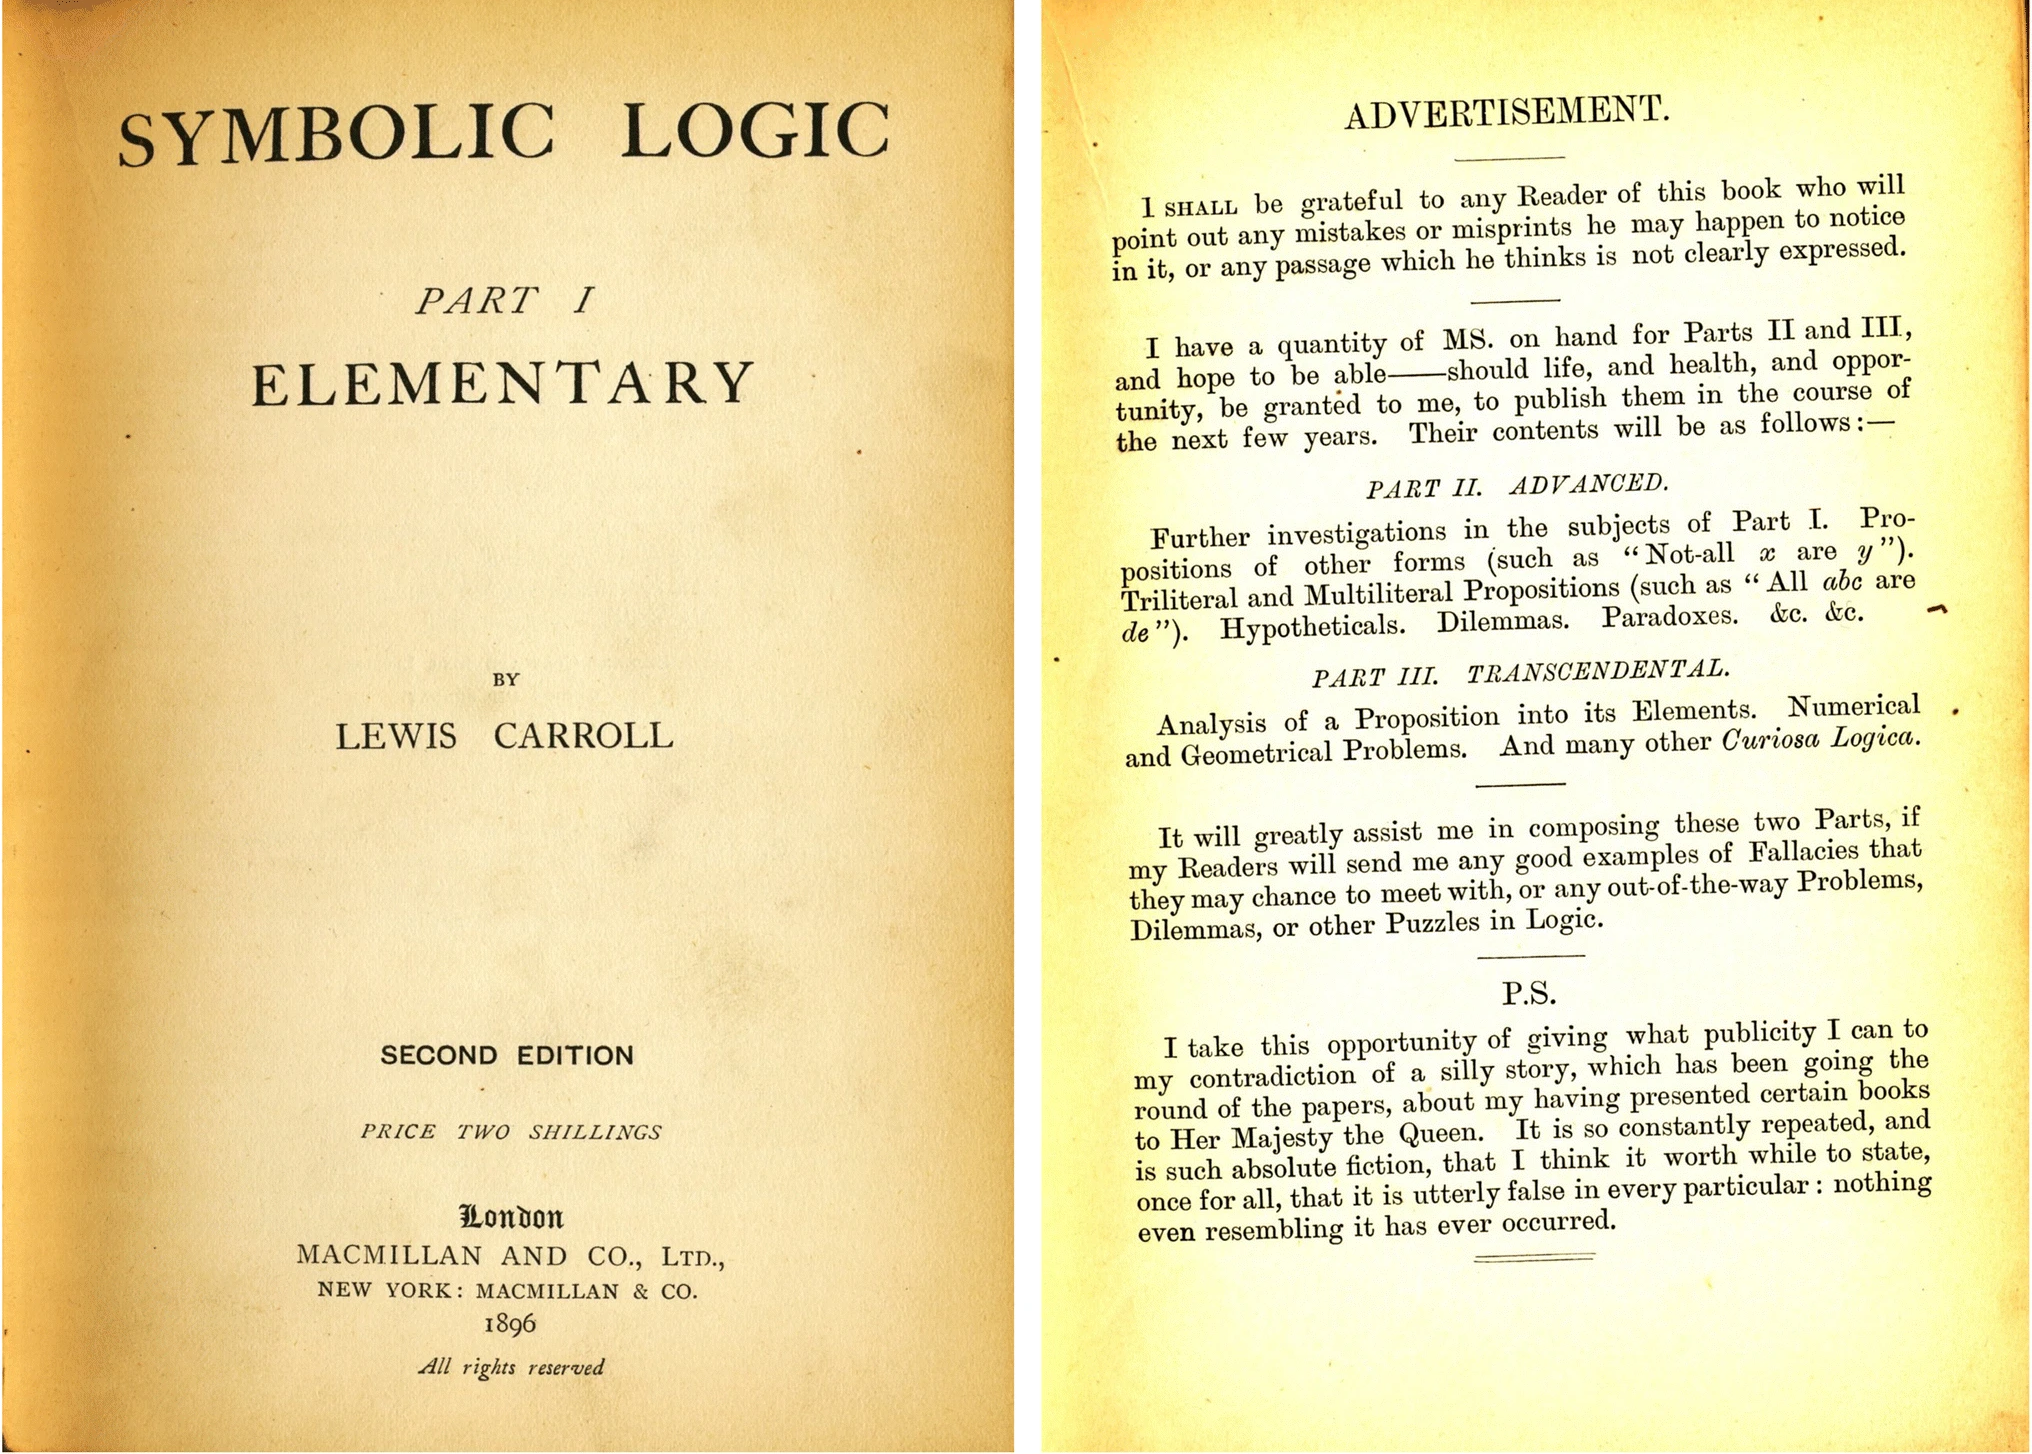
\includegraphics[width= 0.4\textwidth]{4}
		\caption{\small\textit{\color{gocco}Hình $4$.}}
		\vspace*{-10pt}
	\end{figure}
	\begin{figure}[H]
		\vspace*{-5pt}
		\centering
		\captionsetup{labelformat= empty, justification=centering}
		\includegraphics[width= 0.4\textwidth]{5}
		\caption{\small\textit{\color{gocco}Hình $5$.}}
		\vspace*{-10pt}
	\end{figure}
\end{multicols}




